\documentclass{UoNMCHA}
\usepackage[authoryear]{natbib}
\usepackage{array,booktabs} % For nice tables
\usepackage{amsmath,amsfonts,amssymb} % For nice maths
\usepackage{float}
\usepackage{color}
\usepackage{multicol}
\usepackage{enumerate}
\usepackage{listings}
\usepackage{subfig}
\usepackage{hyperref}
\usepackage[parfill]{parskip}   % For replacing paragraph indenting with a newline instead
\newif\ifcomment
\commenttrue
\commentfalse
% Number equations per section
\numberwithin{equation}{section}

\hypersetup{
%    bookmarks=true,         % show bookmarks bar?
%    unicode=false,          % non-Latin characters in AcrobatÕs bookmarks
%    pdftoolbar=true,        % show AcrobatÕs toolbar?
%    pdfmenubar=true,        % show AcrobatÕs menu?
%    pdffitwindow=false,     % window fit to page when opened
%    pdfstartview={FitH},    % fits the width of the page to the window
%    pdftitle={My title},    % title
%    pdfauthor={Author},     % author
%    pdfsubject={Subject},   % subject of the document
%    pdfcreator={Creator},   % creator of the document
%    pdfproducer={Producer}, % producer of the document
%    pdfkeywords={keyword1} {key2} {key3}, % list of keywords
%    pdfnewwindow=true,      % links in new window
    colorlinks=true,       % false: boxed links; true: colored links
    linkcolor=blue,          % color of internal links
    citecolor=blue,        % color of links to bibliography
%    filecolor=magenta,      % color of file links
    urlcolor=blue           % color of external links
}

\definecolor{light-gray}{gray}{0.95}
\definecolor{myblue}{RGB}{20,105,176}
\definecolor{myorange}{RGB}{255,140,0}
\definecolor{mygrey}{RGB}{64,64,64}
\definecolor{MATLABKeyword}{rgb}{0,0,1}
\definecolor{MATLABComment}{rgb}{0.1328125,0.54296875,0.1328125}
\definecolor{MATLABString}{rgb}{0.625,0.125,0.9375}

\lstset{language=Matlab,
    basicstyle=\small\ttfamily,
    keywordstyle=\color{MATLABKeyword},
    %identifierstyle=,
    commentstyle=\color{MATLABComment},
    stringstyle=\color{MATLABString},
    numberstyle=\tiny,
    %numbers=left,
    basewidth=0.5em}
\lstset{
language=C,
numbers=none,
xleftmargin=1cm,
frame=tblr,
classoffset=0,
morekeywords={LED_BUILTIN,HIGH,LOW,OUTPUT,INPUT,INPUT_PULLUP},keywordstyle=\color{myblue},
classoffset=1,
morekeywords={analogWrite,pinMode,write,Serial,begin,print,println,digitalWrite,delay,Stepper,step,setSpeed},	keywordstyle=\color{myorange},
classoffset=0,
commentstyle=\color{mygrey},
breaklines=true,
postbreak=\space //...
}

\firstpage{1}    % Set page number for first page
\UoNMCHAreportNo{ELEC1710 S2  } %Report number
\UoNMCHAyear{ }   % Year
\shorttitle{ELEC1710 - Lab 2} %For odd pages
%%%%%%%%%%%%%%%%%%%%%%%%%%%%%%%%%%%%%%%%%%%%%%%%%%%%
\begin{document}
\title{Lab 2:\\Breadboard Implementation of a 7-segment Display Decoder \\ \ \\
{\small ELEC1710  \\ 
}}
%\author[UoNMCHA]{Student Name}
%\address[UoNMCHA]{
%Student of Mechatronics Engineering,\\
%The University of Newcastle, Callaghan, NSW 2308, AUSTRALIA \\
%Student Number: 3...... \\
%E-mail: \href{mailto:First.Last@uon.edu.au}{\textsf{First.Last@uon.edu.au}}}
%%%%%%%%%%%%%%%%%%%%%%%%%%%%%%%%%%%
\maketitle
\onecolumn

\vspace{-5mm}

\section{Introduction}

When builing an electronic device, whether for electrical, medical or mechatonic engineering projects, it is quite likely you would want to display a numerical value to its users. A simple way to do this is using a 7-segment LED display.

The segments of a 7-segment display are referred to by the letters A to G. Each segment of the display is turned 'on' or 'off' depending on which digit is to be displayed as shown in Figure \ref{fig:7seg}.  Often an eigth segment, referred to as DP, is also available for use as a decimal point to display non-integer numbers.


\begin{figure}[H]
{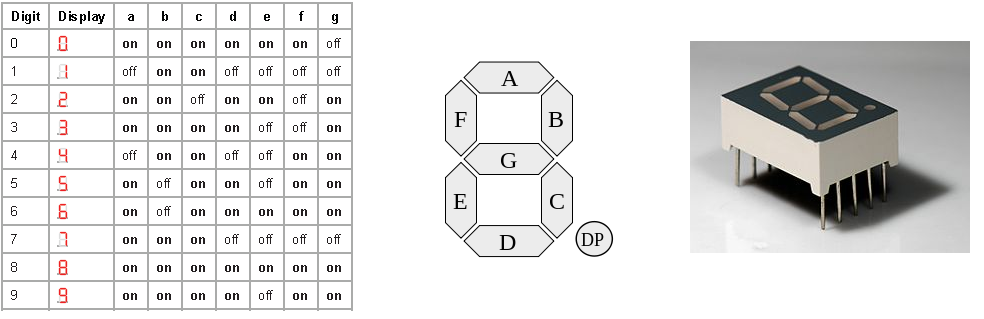
\includegraphics[width=0.9\textwidth]{Figures/Seven-segment-display-Wikipedia2.png}
\caption{7-segment display ({https://en.wikipedia.org/wiki/Seven-segment-display}) To display a '1' the LEDs labelled 'b' and 'c' are turned on while all other LED segments are turned off.
\label{fig:7seg}}}
\end{figure}

In this lab you will implement a pre-designed logic circuit on a breadboard which takes a 4-bit binary number as an input and outputs the appropriate decimal digit on a 7-segment display. Prior to the lab please review the 4-bit binary representation of the decimal numbers from 0 to 9.

\section{Equipment}

This lab will require the following parts:

\begin{itemize}
    \item 1x 7-segment display
    \item 1x CD74HC4511 7-segment display decoder/driver
    \item 7x $330\Omega$ resistors (orange-orange-brown-gold)
    \item 4x $10$k$\Omega$ resistors (brown-black-orange-gold)
    \item 4x Tactile push button switches
    \item Multiple jumper wires
\end{itemize}

\section{7-segment Driver Description}

This lab makes use of the CD74HC4511 BCD-to-7-segment latch/decoder/driver intergrated circuit (IC). This device latches (remembers) binary coded decimal data present on the data input pins (D0, D1, D2 \& D3) and generates appropriate signals on outputs a,b,c,...,f to display a decimal digit on a 7-segment display. The device is called a `driver' because it is capable of supplying the (relatively) high currents required to drive LEDs in a 7-segment display (about 5-10mA, depending on voltage).

The device also contains three control pins:

\begin{itemize}
    \item $\overline{\texttt{LT}}$ - Lamp Test, active low. If low all segments become lit.
    \item $\overline{\texttt{BL}}$ - Blank, active low. If low all segments are switched off.
    \item $\overline{\texttt{LE}}$ - Latch Enable. When this pin is low data on D0-D3 is decoded to a 7-segment number. As this pin goes high the binary data on D0-D3 is internally remembered (latched) and changes on D0-D3 are ignored.
\end{itemize}

The full truth table for the CD74HC4511 is shown in Figure \ref{fig:ttable}.

\begin{figure}[H]
\makebox[\textwidth][c]{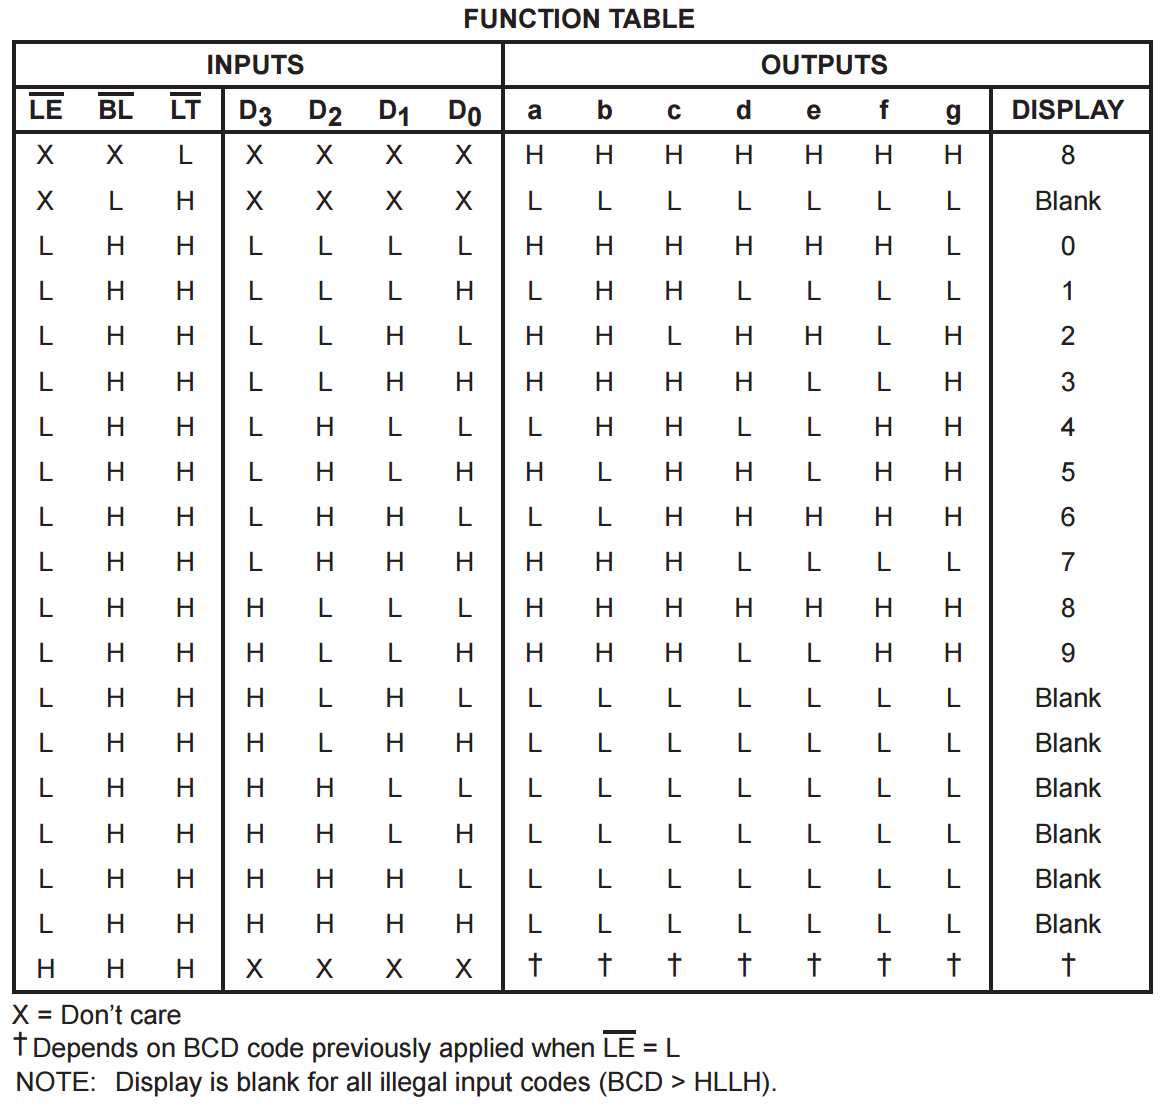
\includegraphics[width=0.7\textwidth]{Figures/CD74HC4511_table}}
\caption{Truth table for the CD74HC4511}
\label{fig:ttable}
\end{figure}

\pagebreak
\section{Procedure}
\begin{enumerate}
    \item Ensure that the power supply module is switched off and that both output voltage jumpers are set to +3.3~V.
    \item Follow the schematic in Figure \ref{fig:schematic} to complete the following steps:
    \begin{enumerate}
        \item Insert the push button switches into the breadboard. It is recommended that they are inserted in a group however space them out enough to facilitate easy operation and removal.
        \item Open the Lab 1 document and find the push button pinout shown in Figures 3 and 4.
        \item Connect one terminal of each switch to the positive supply rail.
        \item Connect the other terminal to GND via a 10k$\Omega$ resistor.
        \item Insert the CD74HC4511 into the breadboard approximately 1cm away from the nearest switch.
    \end{enumerate}
\begin{figure}[H]
\makebox[\textwidth][c]{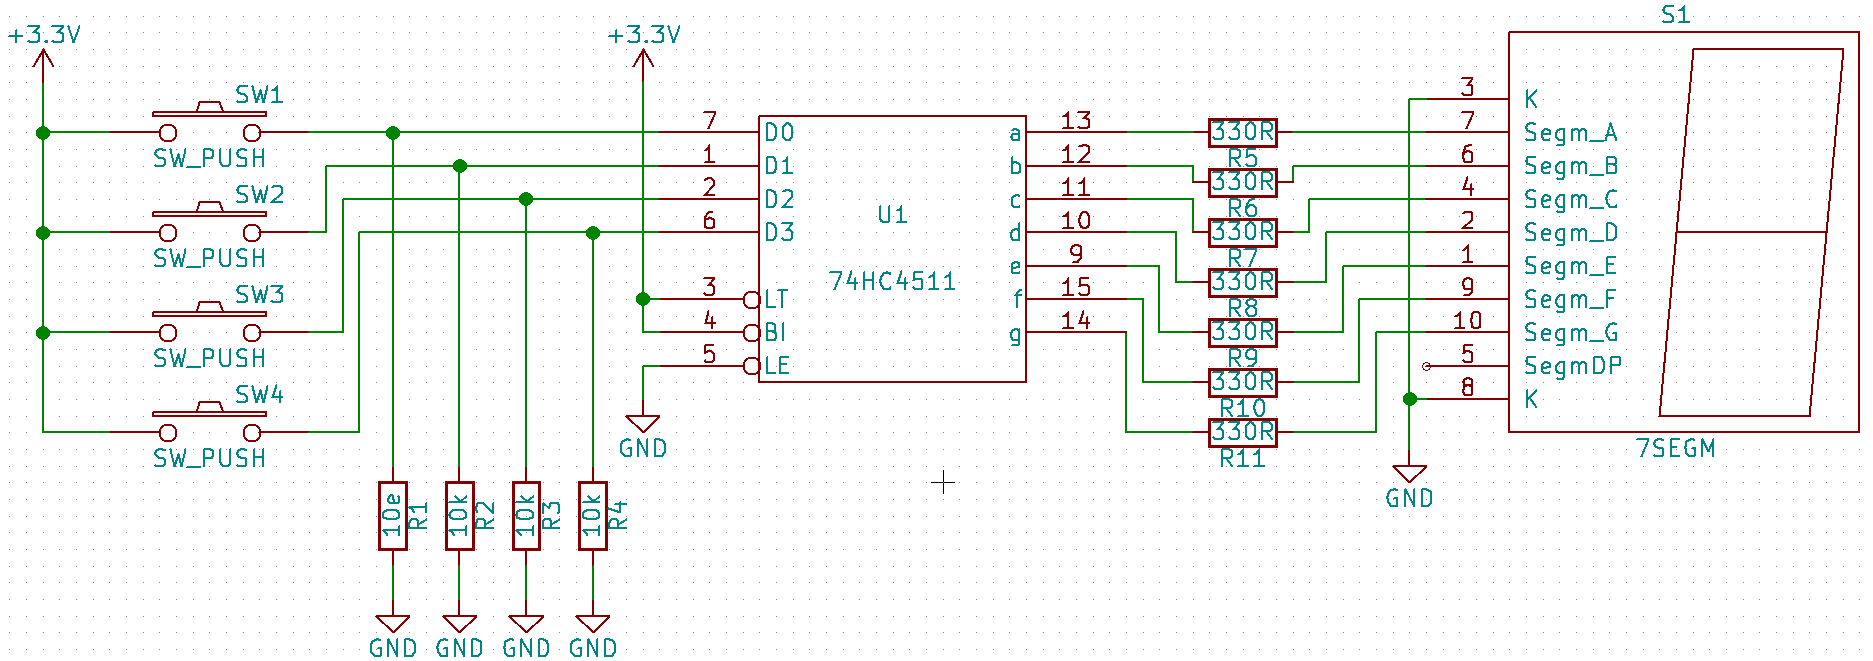
\includegraphics[width=1.0\textwidth]{Figures/schematic}}
\caption{Full circuit schematic}
\label{fig:schematic}
\end{figure}
    \item Observing the schematic in Figure \ref{fig:schematic} and CD74HC4511 pinout in Figure \ref{fig:4511pinout} make the following connections:
    \begin{enumerate}
        \item Connect pin 16 (Vcc) to the positive supply rail
        \item Connect pin 8 (GND) to ground
        \item Connect the four switch outputs to the D0, D1, D2 \& D3 inputs (pins 7, 1, 2, \& 6 respectively) on the CD74HC4511.
        \item Connect $\overline{\texttt{LT}}$ (pin 3) to Vcc
        \item Connect $\overline{\texttt{BL}}$ (pin 4) to Vcc
        \item Connect $\overline{\texttt{LE}}$ (pin 5) to GND
    \end{enumerate}
\begin{figure}[H]
\makebox[\textwidth][c]{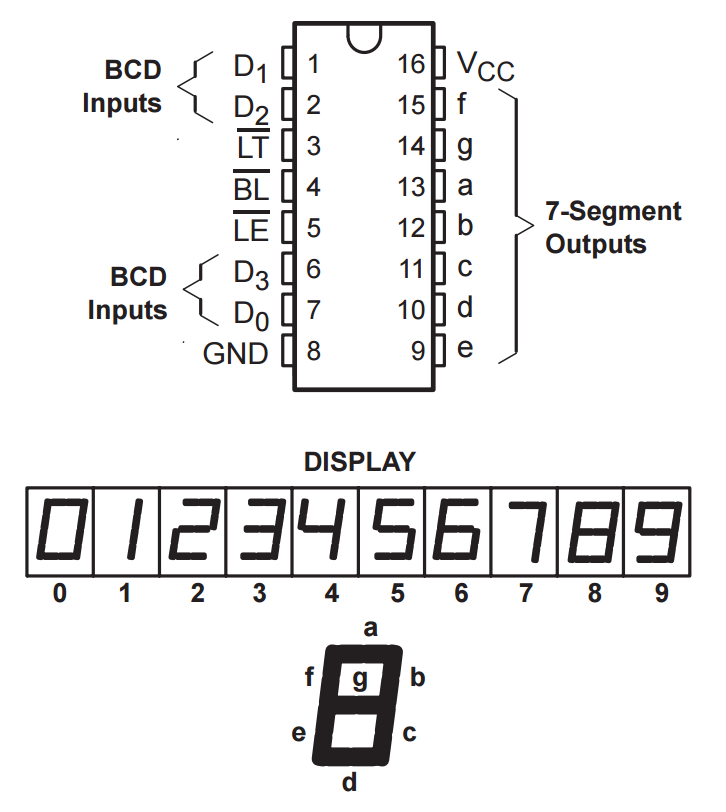
\includegraphics[width=0.5\textwidth]{Figures/CD74HC4511_pinout}}
\caption{CD74HC4511 Pinout}
\label{fig:4511pinout}
\end{figure}
    \item Observe Figure \ref{fig:ssegpinout}. Pins 3 and 8 of the 7-segment display are the common cathode pins, connect each of these to GND with jumper cables.
\begin{figure}[H]
\makebox[\textwidth][c]{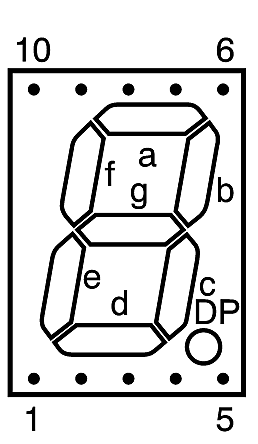
\includegraphics[width=0.25\textwidth]{Figures/sseg_pinout}}
\caption{Pin numbering on the 7-segment display}
\label{fig:ssegpinout}
\end{figure}
\begin{figure}[H]
\makebox[\textwidth][c]{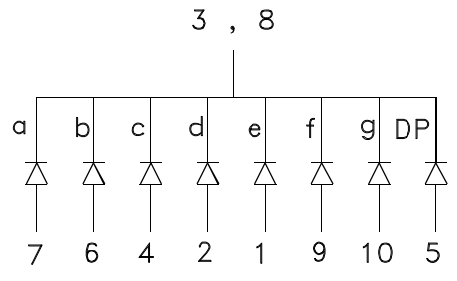
\includegraphics[width=0.5\textwidth]{Figures/ssegpins}}
\caption{Internal schematic of the 7-segment display. Note that the cathode (negative) of each LED is connected to a common point on pins 3 and 8.}
\label{fig:sseginternal}
\end{figure}
    \item Following the schematic in Figure \ref{fig:schematic}, CD74HC4511 pinout in Figure \ref{fig:4511pinout}, 7-segment pinout in Figure \ref{fig:ssegpinout} and 7-segment internal schematic in Figure \ref{fig:sseginternal} connect a $330~\Omega$ resistor from each segment driver pin on the CD74HC4511 (a,b,..,g) to its respective input on the 7-segment display.
    \item Turn the breadboard power supply on and confirm that the display shows a number 0.
    \item Count in binary on the push buttons and ensure that all digits are displayed correctly. \\\textbf{NB:} Entering a number greater than 9 will cause the display to go blank.
    \item Use the Saleae analyser to measure the delay between the input bits changing and the corresponding output appearing. You will have to set the capture rate to maximum (500~MS/s) and use the trigger function on an input pin. Don't capture more than about 5 seconds of data as the lab PC will run out of RAM and possibly freeze.
    
    Compare this measurement with the CD74HC4511's specification of 25~ns. At 500~MS/s the sample period is 2~ns so you can add annotations to the Saleae plot to take measurements with +/- 1~ns accuracy.
\end{enumerate}



\end{document}